\newpage
\chapter{Methodology}

As the problem explained in the \textit{Problem statement} chapter, there are two mainly requirements of this thesis:

\begin{itemize}
	\item When the \textit{redirection} is activated by the administrator for some reasons(Fire alarm, terrorist attack, etc. ), all the HTTP requests will be redirected to a specified target IP, which is the web server defined below.
	\item A running web server, which will return the direct connected network device of the client.
\end{itemize}

Hence, this chapter will describe the principles about how to achieve the target.

\section{Network Protocols}

This section will describe the principle of related network protocols.

\subsection{OSI \& TCP/IP models}

\textbf{OSI}, \textit{Open System Interconnect}, is a reference model, which is developed by ISO and CCITT, providing the framework of a functional structure for telecommunication systems or computing systems. It is established from low to high: Physical Layer, Data Link Layer, Network Layer, Transport Layer, Session Layer, Presentation Layer and Application Layer.

\begin{figure}[!ht]
	\caption{OSI model.}
	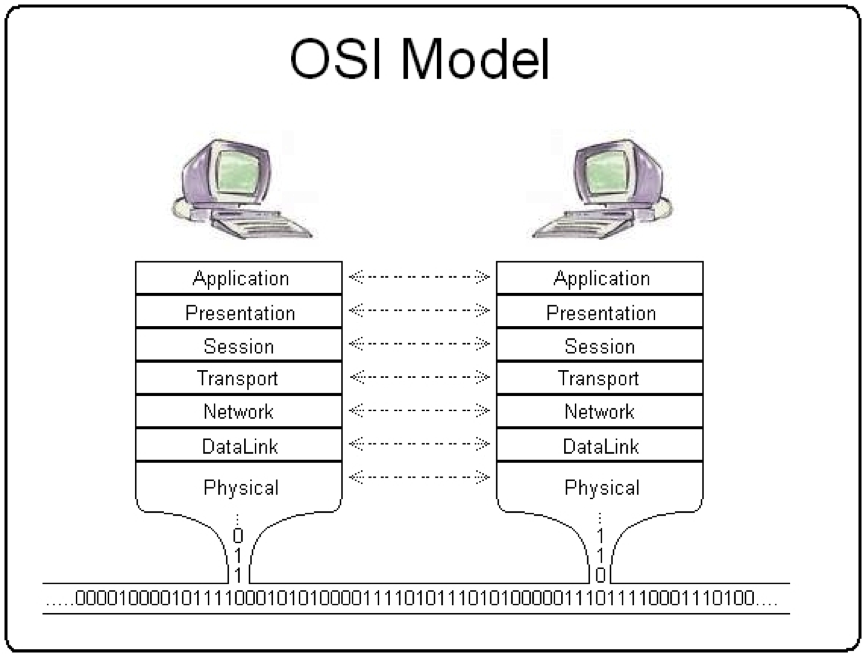
\includegraphics[width=\textwidth]{images/osi_model}
\end{figure}

\textbf{TCP/IP} is a set of communication protocols, using to implement a network interconnection. It is the kernel for Internet network architecture in\cite{rfc1213}. The reference model is divided into four levels, these were: Host-to-Network Layer, Internet Layer, Transport layer and the Application layer.  

\subsubsection{Reference Model Comparison}

The common attributes:

\begin{itemize}
	\item OSI reference model and TCP / IP reference models use the structure of hierarchy.  
	\item Both of them provide connection-oriented service and connectionless service.  
\end{itemize}

The different attributes(see also the table below): 

\begin{itemize}
	\item OSI use seven-layer model, but TCP / IP is a four-layer structure.  
	\item Host-to-Network Layer is actually no real definition in TCP / IP reference model, has just some conceptual descriptions. But OSI reference model is not only divided the two layer (Physical Layer and Data Link Layer), but also are very detailed in the function of each layer.  
	\item OSI model is designed before any protocols were developed, so it has universality. TCP / IP model has first the set of protocols, after that it built the model, so it does not apply to non-TCP / IP networks.  
	\item The concept of OSI reference model is the clear structure, but is too complex. TCP / IP reference model is not clear on the services, interfaces and the difference of protocols. 
\end{itemize}

\begin{table}[h]
\begin{longtable}{| c | p{8em} | c | p{12em} |}
\hline
\textbf{OSI} & \textbf{Protocol data unit} & \textbf{TCP/IP} & \textbf{TCP/IP protocols} \\ \hline
Application & Data & Application & TFTP, HTTP, SNMP, FTP, SMTP, DNS, Telnet, etc. \\ \hline
Presentation & Data &  & No agreement \\ \hline
Session & Data & & No agreement \\ \hline
Transport & Segment (TCP)/ Datagram (UDP) & Transport & TCP, UDP \\ \hline
Network & Packet & Internet & IP, ICMP, OSPF, EIGRP, IGMP \\ \hline
Data link & Frame & Host-to-Network & SLIP,CSLIP, PPP,MTU \\ \cline{1-2} \cline{4-4}
Physical & Bit & & ISO2110, IEEE802, IEEE802.2\\
\hline
\end{longtable}
\caption{Protocols refer to OSI and TCP/IP layers}
\end{table}

\subsection{SNMP (Simple Network Management Protocol)}

\subsubsection{Overview}

As the network scale increases, it becomes more difficult for network administrators to monitor the status of all devices in a short timeline, to discover and repair the fault.  

SNMP is short term for Simple Network Management Protocol, SNMP is defined as the application protocol for the management services on network. For the first time in August 1988 defined by the Internet Engineering Task Force (IETF) research team in order to solve the problems with the Internet router administration. Soon it reached a formal standard in RFC1157\cite{rfc1157}. SNMP is composed of a series of protocols and specifications, which provide a method for collecting network management information from devices on the network. It collects data from managed devices in two ways: First is polling (polling-only) method, and the second is the interrupt-based approach. These protocols are supported by many typical network devices such as routers, hubs, bridges, switches, servers, workstations, printers, modem and other network components and devices.

All SNMP messages is received via UDP port 161, only Trap information using UDP port 162.

\begin{figure}[!ht]
	\caption{SNMP communication principles diagram}
	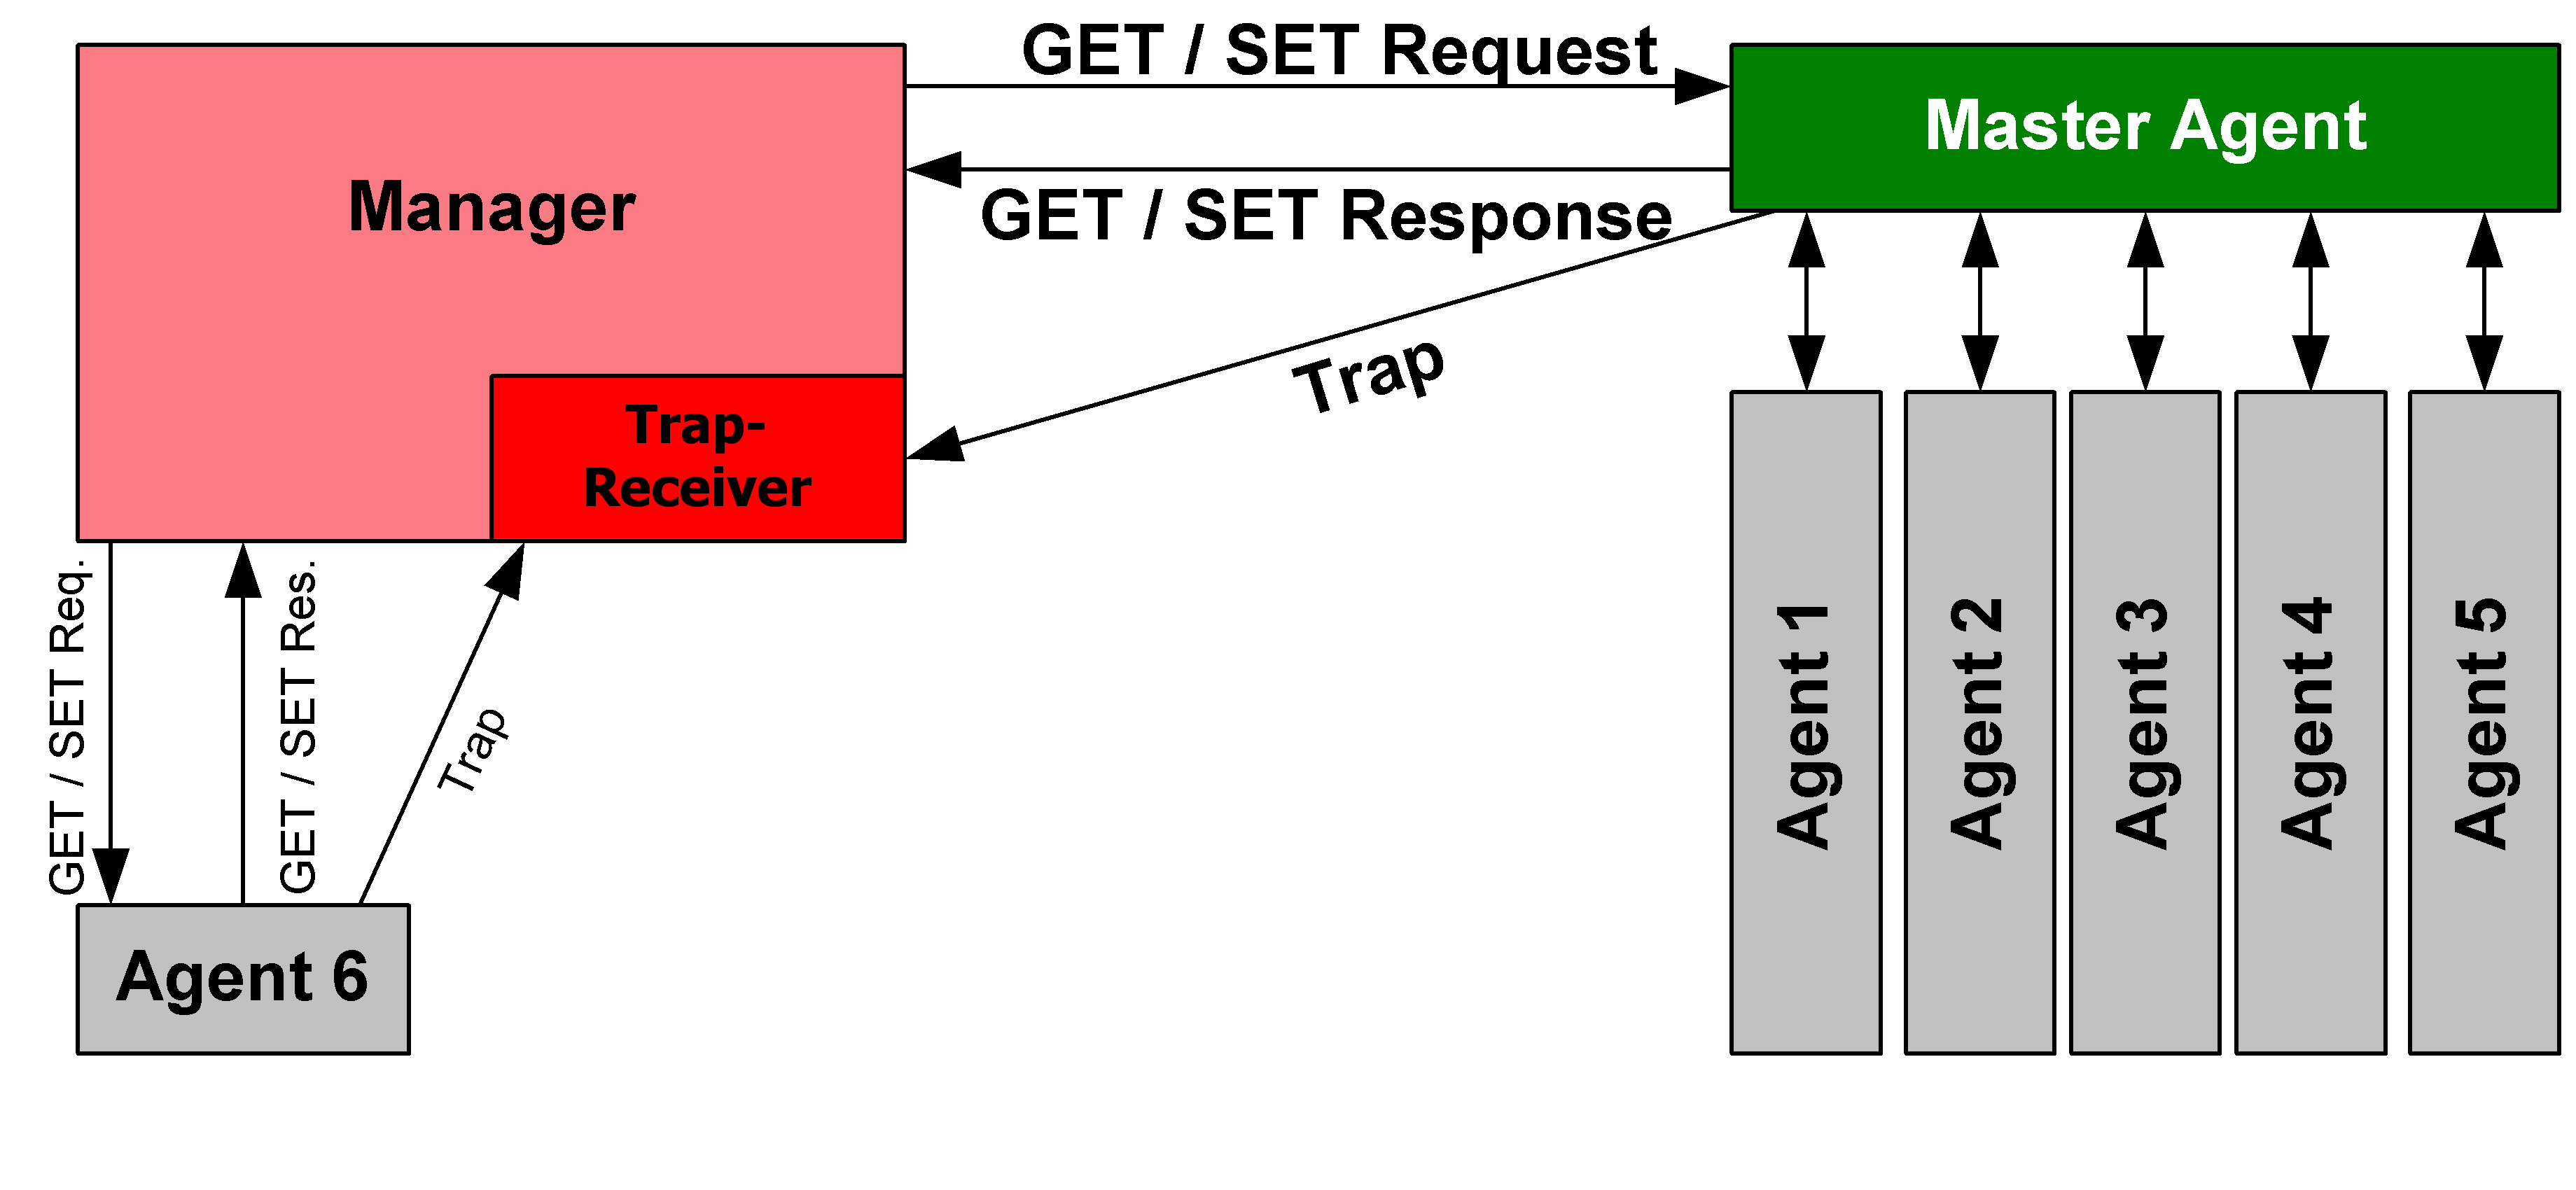
\includegraphics[width=\textwidth]{images/SNMP_communication_principles_diagram}
\end{figure}

\subsubsection{SNMP Network Architecture}

SNMP network architecture consists of three parts: \textit{NMS}, \textit{Agent} and \textit{MIB}.

\paragraph{NMS}

NMS is the network manager, takes usage of SNMP for network device management and monitoring system. NMS refers to a dedicated server for network management, it also refers to a device executed management functions of an application.  
NMS can send a request to the Agent, select or modify one or more of the specific parameter values. At the same time, NMS can receive Trap information from Agent sends, in order to learn the current status of the managed devices.  

\paragraph{Agent}

Agent is an application module of device in network, used to maintain the managed device information and to respond NMS's request, to report management data to the NMS, which sends the request.  

After Agent receives request information from NMS, it completes the query or modify operation and sends the operation result to NMS, in order to complete the response. Meanwhile, when the device has malfunction or other event, Agent will send initiatively trap information to the NMS and notice the change of current status on device.  

\paragraph{MIB}

Any managed resource can be represented as an object, called the managed object. MIB in\cite{rfc1493}\cite{rfc4188} is a collection of managed objects. It defines a set of properties for managed objects: Object name, object access permissions and object data types, etc.  

Each Agent has its own MIB. MIB also can be seen as an interface between the NMS and the Agent, through this interface, NMS can make 'read' or 'write' operations to each managed object in Agent, in order to achieve the purpose of managing and monitoring devices.  

MIB stores data within a tree structure. The node of the tree represents a managed object, it can use a path starting from the root to uniquely identify, and this path is called OID.

\begin{figure}[!ht]
	\caption{MIB-II subtree. This figure show the tree structure of MIB.}
	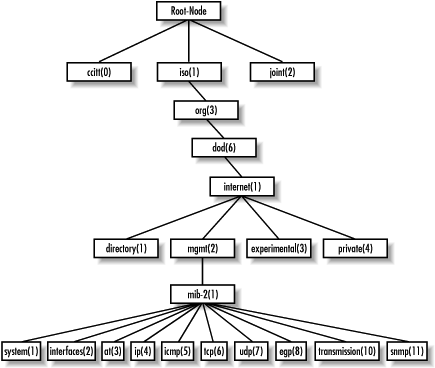
\includegraphics[width=\textwidth]{images/MIBsubtree}
\end{figure}

\subsubsection{SNMP Version}

\paragraph{SNMPv1}

\textit{SNMPv1} is the initial version of the SNMP, providing minimal network management capabilities. The SNMPv1's SMI and MIB are almost insecure, due to a large number of security vulnerabilities.  
SNMPv1 uses community names for authentication. The characteristic of community names like a password to restrict the access to the Agent of the NMS. If SNMP packets with community names have not been approved in the NMS or Agent, the packets will be discarded.  

\paragraph{SNMPv2}

\textit{SNMPv2} also uses community names for authentication. At the same time it is compatible with SNMPv1 and adds several features comparing to SNMPv1:
\begin{itemize}
	\item It Provides more operation types (Get Bulk operations, etc.)
	\item Support for the more data types (Counter32 etc.)
	\item It Provides richer error codes, more details to analyse and distinguish error
\end{itemize}

\paragraph{SNMPv3}

\textit{SNMPv3} has been enhanced primarily in terms of security, it uses USM und VACM technology.  

\textbf{USM}(\textit{User-based Security Model}) provides authentication and encryption capabilities, \textit{USM} introduces the concept of user names and groups, set the authentication and encryption features.  

\textbf{VACM}(\textit{View-based Access Control Model}) determine the user, whether is allowed access, specific MIB objects and access method, \textit{VACM} technology defines five elements: the group, security level, contexts, MIB view, access policy, these elements control access privileges, it decides whether the user is allowed for access.

\subsubsection{SNMP Operations}

\textit{SNMP} support for multiple operating, mainly for the following basic operations:

\begin{description}
	\item[Get] NMS use the operation to obtain one or more parameter values from the Agent.
	\item[GetNext] NMS get to the next parameter value of one or more parameters from the Agent.
	\item[Set] NMS set up one or more parameter values in the Agent.
	\item[Response] Agent returns one or more parameter values. This action is in response to the preceding three operations.
	\item[Trap] Agent sends actively the operation to inform the NMS, What happened.
\end{description}

When performing the first four operations, the device uses the UDP protocol in port 161 to send packets, when performing Trap operation, the device uses the UDP protocol in port 162 to send packets. Hence using a different port number, a device can act simultaneously as Agent and NMS.

\subsubsection{SNMP Technical advantages}

\textit{SNMP} has the following technical advantages\footnote{Definition and Explanation about SNMP: \url{https://www.techopedia.com/definition/5473/simple-network-management-protocol-snmp}}:  

\begin{itemize}
	\item Based on the standard protocol TCP / IP, transport layer generally use UDP (User Datagram Protocol).  
	\item Automated Network Management. The network administrators can use SNMP on the network to retrieve information, modify information, find fault, complete fault diagnosis, plan capacity and report.  
	\item Shield the physical differences in different device, to achieve automatic management of products from different vendors.  
	\item SNMP provides only the most basic feature, which gives independence in the management tasks, physical properties of the managed devices and the actual network type, in order to achieve the management of devices for different vendors.  
	\item SNMP have simple mode of request - response, active notification methods, timeout and retransmission mechanism.  
	\item Less packet type, simple format of packet is easy to be resolved and to be implemented.  
	\item SNMPv3 provides the security mechanisms of authentication and encryption, as well as the access control capabilities based on user and view, to enhance security.
\end{itemize}

\subsection{MAC Address}

\textbf{MAC Address} means \textit{Media Access Control} or \textit{Medium Access Control}. Or it is called the physical address, hardware address, is used to define the location of network device. In the OSI model, the network layer (OSI Layer 3) is responsible for the IP address; the data link layer is responsible for the MAC address. Therefore, a media interface has a MAC address and an IP address in network. The network interface controller (NIC) determines the MAC address, and it is fixed. (Belongs to the device)  

\textit{MAC address} used hexadecimal digits separated by hyphens (-) or by colons (:) , a total of six bytes (48 bits). Actually \textit{MAC address} is the adapter address or adapter identifier EUI-48. It is divided into the first three octets and the following three octets:  

\begin{itemize}
	\item The first three octets, is called Organizationally Unique Identifier, namely OUI. It is assigned to different manufacturers, which have registered in IEEE, to distinguish the devices of the different manufacturers.
	\item The following three octets, is assigned by the manufacturers themselves, called Extended Identifier. For the same manufacturer, it is also different.
\end{itemize}

Speaking of the \textit{MAC address}, we have to speak about IP address (see the next section).

To complete the communication, IP addresses working on the network layer, the packet is forwarded from one network to another network; MAC addresses are based on the data link layer, a frame is transmitted from one node to another one in the same link. In a stable network, IP addresses and MAC addresses are a pair. So IP addresses and MAC addresses are corresponding to each other. This mapping between IP addresses and MAC addresses has to be done by the \textit{ARP} (\textit{Address Resolution Protocol}).  

The difference between the MAC address and IP address:  

The same with MAC address and IP address is sole (meaning?), but the different characteristics are:  

\begin{itemize}
	\item On the same device or a computer, the change and customisation of the IP address is easy (but it must be unique). The MAC address was made by the manufacturer, it generally cannot be changed.
	\item Different length. The length of IP address is 32 bits, MAC address is 48 bits.
	\item Different assignment rules. IP address based on the network topology, MAC address based on the manufacturer.
	\item Different OSI layer for the addressing.
\end{itemize}

\subsection{IP}

\textbf{IP} is the abbreviation for Internet Protocol, meaning "interconnection protocol between networks". In the Internet, it is a set of rules to make all devices, which are connected to the Internet network, compatible with each other for communication. The devices should comply with the rules. Any system manufacturers of a device, as long as it complies the IP, could be interconnected to the Internet. Because of IP, the Internet was able to have rapid development and became the world's largest open communication network.  

\subsubsection{IPv4 vs. IPv6}

\textit{IPv4}, Internet Protocol version 4 (IPv4) is the fourth version of the Internet Protocol (IP), It is also the first to be used widely, which is the basis of protocol in the current Internet. In 1981, Jon Postel defined the IP in RFC791.  

IPv4 runs on a variety of the bottom network. In local area network, an Ethernet used it most commonly. But its biggest problem is the limited place of network address.  

\textit{IPv6}, Internet Protocol version 6 is the recent version of the Internet Protocol (IP). IPv6 is the next generation IP protocol, which was designed by IETF (Internet Engineering Task Force), to replace the current Internet Protocol version (IPv4).  
Compared with IPV4, IPV6 has the following advantages:  

\begin{itemize}
	\item IPv6 has a larger space for IP address. The length of IPv4 address is 32 bit, that is $ 2^{32} - 1 $ addresses. IPv6 is 128 bit, has $2^{128} - 1 $ addresses.
	\item IPv6 uses the smaller routing tables. The assignment of IPv6 address follows Aggregation principle. It makes the Router with a Entry record to represent lots of the subnet, in order to reduce the length of the routing table and improve the speed of packet forwarding in router.
	\item IPv6 enhances the support of Multicast and Flow Control, greatly improving for Quality of Service (QoS).
	\item IPv6 adds the support of the auto-configuration. This is an improvement and expansion of DHCP, to make the network (especially local area network) management more convenient and faster.
	\item IPv6 has a higher level of security. Using IPv6, the users encrypt data at the network layer and check the IP packet.
\end{itemize}

\subsubsection{IP Address}

\textbf{IP} provides a uniform address format, named the Internet Protocol address. It assigns a logical address for each network and each host on the Internet, in order to mask the differences in the physical address. Each device in network needs to have an IP address for normal communication. Then the "IP address" is equivalent to "phone number", and the router acts as "program-controlled switch."  

An IP address is a 32-bit binary number; it is usually divided into four times "8-bit binary number"---four bytes. IP address is usually the dotted decimal notation, the form as (a.b.c.d), in which a, b, c, d is a decimal integer number from 0 to 255.  

\subsubsection{IP Address Type}

The type of IP address is composed of public address and private address.  
The Internet NIC (Internet Network Information Center) is responsible for the public address. The IP address is assigned to the organizations, which will register or apply to the Inter NIC. It gains access directly to the Internet with it. Private address is a non-registered address, used exclusively for the internal organization.  

\subsubsection{IP Address Classification}

IP address according to different network ID is divided into five types, A class to - E class.  

A, B, C class is uniformly distributed Internet NIC in worldwide, D class and E class are the special addresses.  

Class D is to be called multicast address.

\begin{table}[h]
\begin{longtable}{| p{4em} | p{6em} | p{6em} | p{7em} | p{9em} |}
\hline
\textbf{category} & \textbf{The maximum number of network} & \textbf{IP address range} & \textbf{The maximum number of hosts} & \textbf{Private IP address range} \\ \hline
A & 126($ 2^7-2 $) & 0.0.0.0-127.255.255.255 & 16777214 & 10.0.0.0-10.255.255.255 \\ \hline
B & 16384($ 2^{14} $) & 128.0.0.0-191.255.255.255 & 65534 & 172.16.0.0-172.31.255.255 \\ \hline
C & 2097152($ 2^{21} $) & 192.0.0.0-223.255.255.255 & 254 & 192.168.0.0-192.168.255.255 \\ \hline 
\end{longtable}
\caption{Categories of IP address}
\end{table}



Special addresses are listed below:

\begin{itemize}
	\item Each byte is 0 ("0.0.0.0"), corresponding to the current host
	\item Each byte is 1 ("255.255.255.255"), corresponding to the broadcast address of current subnet
	\item IP addresses cannot be a decimal "127" at the beginning, from 127.0.0.1 to 127.255.255.255 for the Loop Test. Such as: 127.0.0.1 represents the local IP address, using the "http://127.0.0.1" to test the configuration of the Web server in machine
\end{itemize}

\subsubsection{IP Address in LAN or WLAN}

In a LAN or WLAN, there are two special IP addresses, a network number and a broadcast address. Network number is the address for addressing, which represents the whole network itself; another is the broadcast address, which represents all of the host network. Network number is the first IP address in the segment, broadcast address is the last IP address in the segment, and these two addresses are not configured on the host. For example, in this segment 192.168.0.0,Subnet Mask is 255.255.255.0, Network number is 192.168.0.0, and the broadcast address is 192.168.0.255. Host IP address can be configured only from 192.168.0.1 to 192.168.0.254.  

\subsection{HTTP}

\textbf{HTTP} is \textit{HyperText Transfer Protocol}, which is the most widely used network protocol on the Internet. All WWW documents must comply with this standard. Original HTTP was designed to provide a method to publish and receive HTML pages. World Wide Web Consortium and the Internet Engineering Task Force cooperatively researched and released a series of RFC, including the famous RFC 2616 for the definition of the HTTP 1.1.   

HTTP uses a request - response model in the client-server computing model. After a client establishes a connection to a server, it sends a request to the server, the format of the request method is Uniform resource identifier(URI) and protocol version. The server receives the request, then give the response information. Its format is a status line, including protocol version and a code of success or error. The returned information from server is received by client, it is displayed on the user's screen through the browser. Afterwards aborts the connection.

\subsection{DHCP}
\textbf{DHCP}, \textit{Dynamic Host Configuration Protocol} is a local area network protocol; typically it is used in large-scale local area network environment. The concentrated management and assignment of the IP address is the main task, to verify that the host can get a dynamic IP address, Gateway address, DNS server address and other relevant information, and enhance the utilization of the IP address.  

DHCP protocol uses a client - server model, it has three mechanisms for the assignment of IP address:

\begin{description}
	\item[Automatic Allocation] DHCP server allocates a permanent IP address for the host.
	\item[Dynamic Allocation] DHCP server allocates the IP address with time limited for the host, as time expires, it can be used by other hosts.
	\item[Manual Allocation] DHCP server allocates the IP address by the network administrator for the host.
\end{description}

DHCP uses UDP as a transport protocol. The host sends a request message to the DHCP server in 67 port, DHCP server gets the response to the host's 68 port.

\subsection{ICMP}

\textbf{ICMP}, \textit{Internet Control Message Protocol}, is a connection-oriented protocol, it was used between hosts and routers to deliver control messages, including the reporting errors, the exchange limited control and status information.  

The main functions of ICMP are listed below:

\begin{itemize}
	\item Detect the remote host, if it exists.  
	\item Establishment and maintenance of the routing information.  
	\item ICMP Redirect  
	\item Flow Control
\end{itemize}

\textit{ping} and \textit{traceroute} are the most common commands based on ICMP. 

\section{Network Devices}

This section describes the network devices used in this thesis.

\subsection{Common types of devices}

\subsubsection{Router}
Router, also known as the gateway device, is used to connect a summary of logically separate networks. The logical network represents an independent network or subnet. When the data transmits from one subnet to another subnet, it can be redirected by routing function of the router. According to the situation of channel, it will automatically select and set routes for the best path in order to send packages. Therefore, the router has the function of determining the network address and select IP path. It can establish a flexible connection in the environment of multiple networks interconnection, though completely different data packets and media access method to connect the various subnets. 

Wireless Router is a router with wireless coverage capabilities, it is mainly used for Internet access and wireless coverage. In the market, popular wireless routers generally supports four kinds of access mode: static xDSL / cable, dynamic xDSL / cable, PPPoE. It also has some other network management functions, such as DHCP service, NAT firewall, MAC address filtering and more. 

The main difference between router and switch: switch works in the second layer of the OSI reference model (Data Link Layer),  but the router in the third layer (Network Layer). This difference determines that the router and switch need to use the different control information in the process of information transmission, so the way to achieve their functions is different. 

\subsubsection{Switch}

The switch provides an exclusive path for the electrical signal, which transfer through the switch for any two nodes in network. The most common is the Ethernet switch.  

The switch works in the second layer (Data Link Layer) of the OSI reference model. The CPU of a switch forms a MAC table through the MAC address and the corresponding port, when each port on the switch is successfully connected. Inside these communications, it sends the packet for the MAC address only by its corresponding port, instead of all ports.  

The switch manages the data transmission between the multiple ports at simultaneous time. Each port can be registered as a separate physical network segment. The network devices, which connects to the switch, use the bandwidth alone, without the other devices to share.

\subsubsection{AP}

\textbf{AP}, \textit{Access Point}, AP is equivalent to a bridge between wired network and wireless network, using the main technology of the 802.11x series in \cite{rfc5416}\cite{Siddhartha2002} . Its main task is to connect each client of wireless network together, and then it is connected to the Ethernet. AP used mainly for home broadband, company-internal network, large buildings and Campus Network, etc. The distance coverage of wireless ranges from tens of meters to hundreds of meters.  

Functions: 

\begin{description}
	\item[Repeat] It improves the wireless signal amplification between two wireless APs, such that the remote client can receive a stronger wireless signal.  
	\item[Bridge] two Communication endpoints are connected by two wireless APs for data transmission. For example, usually it is selected by the AP as bridge for the communication of two wired LANs.  
	\item[Master-slave mode] it allows one point connection to multipoint for the management of sub-network.  
\end{description}

\subsubsection{Repeater}
Repeater could be considered as an signal strength reinforcement device.

\subsection{Devices used in the thesis}

\subsubsection{ProCurve switch}
The ProCurve Series Switches are multi-port switches that can be used to build high-performance switched workgroup networks. These switches are store-and-forward devices that offer low latency for high-speed networking.

The ProCurve switch has an option: Hide its IP address on network. When it is activated, no IP will be assigned to it. But even when this option is deactivated, its IP address can not be found some times.

\subsubsection{ASUS RT-N16}
\textit{ASUS RT-N16} is Multi-Functional Gigabit Wireless N Router with USB storage,printer and media server. Powerful CPU provides a high-performance throughput. It could be used as a router, a repeater or an AP.

A disadvantage of \textit{ASUS RT-N16} is that, all the media interfaces of this device has the same MAC address and media interface. It's special setting of ASUS router, so there is no way to distinguish the media interface.

\subsubsection{Convert Macintosh Computer to Router}

Because that lack of network devices, two Macintosh computers are converted to SNMP supported routers.

The operating system running on Macintosh computers names OS X, based on FreeBSD. It is also an Unix-like operating system. A Macintosh computer with an OS X system could be converted to a router, if corresponding software are installed and configured.

\paragraph{Activate Internet share}
At the \textit{System preference} of OS X (Tested on OS X 10.11, El Capitan), the \textit{Internet share} could be activated. 

\textit{IP forwarding}, also called \textit{Internet routing} is a process used to determine which path a packet or datagram can be sent. While activating, the \textit{net.inet.ip.forwarding} ks set to 1 automatically, and it will be reset to 0 when deactivated.

\paragraph{Launch SNMP service}

The configuration of SNMP is stored in \textit{/etc/snmp/snmp.conf}.

Step 1. Backup the /etc/snmp/snmp.conf file.

Step 2. Modify the /etc/snmp/snmp.conf file: \footnote{How to activate SNMP on Mac OS \url{http://kb.paessler.com/en/topic/41843-how-do-i-activate-snmp-on-mac-os-in-order-to-monitor-it-with-prtg}}\footnote{SNMP unter Mac OS X 10.8 Mountain Lion aktivieren \url{https://blog.emeidi.com/2013/06/09/snmp-unter-mac-os-x-10-8-mountain-lion-aktivieren/}}

\begin{lstlisting}[language=bash]
sudo vim /etc/snmp/snmpd.conf
\end{lstlisting}

\begin{lstlisting}[language=bash]
#Allow read-access with the following SNMP Community String:
rocommunity public

# all other settings are optional but recommended.

# Location of the device
syslocation data centre A

# Human Contact for the device
syscontact SysAdmin

# System Name of the device
sysName SystemName

# the system OID for this device. This is optional but recommended,
# to identify this as a MAC OS system.
sysobjectid 1.3.6.1.4.1.8072.3.2.16
\end{lstlisting}

Step 3. Launch SNMP service.

\begin{lstlisting}[language=bash]
$ sudo launchctl load -w /System/Library/LaunchDaemons/org.net-snmp.snmpd.plist
\end{lstlisting}

This command line will activate the SNMP service in Macintosh computer.

After that, test it using command 
\begin{lstlisting}{language=bash, caption={Run snmpwalk on localhost computer}}
snmpwalk -v 2c -c public localhost
\end{lstlisting}

If the SNMP service is launched successfully, it will list all informations in SNMP.

\section{Redirection}

As explained before, when the redirection is activated, all the HTTP requests will be redirected to a specified web server. There are different ways to achieve this target, but it is also plattform-dependent. This thesis choose \textit{PF}(explained below) as the redirection tool, it is because that the operating system of router is OS X, which is base on FreeBSD.

\subsection{iptables}

The command \textbf{iptables}\footnote{iptables official website: \url{http://www.netfilter.org/}} is the userspace command line program used to configure the Linux packet filtering rule set since Linux 2.4.x, it's targeted towards system administrators.

The iptables could also be used to configure the \textit{Network Address Translation}, because the \textit{NAT} is configured from the packet filter.

\subsection{PF}

\textbf{PF} means \textit{Packet Filter}, is added to FreeBSD since 5.3. PF is a full-featured and complete firewall that has optional support for ALTQ (Alternate Queuing), which provides Quality of Service.\footnote{PF official website: \url{https://www.freebsd.org/doc/handbook/firewalls-pf.html}}
\footnote{pf.conf manual page in Mac Developer Library: \url{https://developer.apple.com/library/mac/documentation/Darwin/Reference/ManPages/man5/pf.conf.5.html}}

\footnote{PF and PFCTL in FreeBSD official website:\\ 
	PFCTL: \url{https://www.freebsd.org/cgi/man.cgi?query=pfctl&sektion=8\\}
	PF: \url{https://www.freebsd.org/cgi/man.cgi?query=pf&sektion=4}}

\textbf{PFCTL} means \textit{Packet Filter ConTroLler}, is used to control the \textit{Packet Filter}. It has a lot of parameters and functions, but this thesis does not require them all. The necessary functions are listed below:

\subsubsection{Flush}

This will flush the loaded rules from PF.

\begin{lstlisting}
pfctl -F <modifier>
\end{lstlisting}

There are nine possible modifiers: \textit{nat}, \textit{queue}, \textit{rules}, \textit{states}, \textit{Sources}, \textit{info}, \textit{Tables}, \textit{osfp} and \textit{all}. Actually, the \textit{PFCTL} in this project redirection uses only the \textit{nat} modifier, \textit{pfctl -F nat} will flush all the NAT rules, and the other rules will remain.

But for simple, only the \textit{pfctl -F all} is used, to flush all the rules.

\subsubsection{Enable / Disable}
Package filter could be disabled, using the following command:

\begin{lstlisting}
pfctl -d
\end{lstlisting}

or enable it using the following command:
\begin{lstlisting}
pfctl -e
\end{lstlisting}

\subsubsection{Load rules}

The rules of \textit{pf} could be stored in a configuration file. By default, the file is \textit{/etc/pf.conf}. The following command will load the rules:

\begin{lstlisting}
pfctl -f <configuration file>
\end{lstlisting}

The \textit{configuration file} could be another PF configuration file \textit{shells/pf.conf} contains the rules about redirection. 

\begin{lstlisting}[caption={Sample of pf.conf}]
bridge_if = "bridge100"
server_ip = "192.168.2.1"
protos = "{tcp}"
rdr on $bridge_if inet proto $protos from any to any port 80 -> $server_ip port 80
\end{lstlisting}

\textit{bridge\_if} is the name of bridge interface of Macintosh computer. When \textit{Internet share} is activated, a virtual media interface will be created. This is the \textit{bridge} between two real network interfaces.

\textit{server\_ip} is the target of redirection.

\textit{protos} is abbreviation of \textit{protocols}. Only the packet of corresponding protocols will be redirected.

\textit{rdr} controls the redirection.

\section{Flooding Algorithm}

\textit{Flooding algorithm} is used to locate the client device, it will find out the direct connected device of the client. The core of \textit{Flooding algorithm} is quit simple: the whole network has a root device, which will be queried first. If the target client device is connected to it, the locating process is over, the result will be returned and shown to the client. Otherwise, the \textit{LoYiW} process will query all the sub devices of the root device one by one recursively, until the client device is found or all the sub devices have been queried.